\documentclass{article}
\usepackage[utf8]{inputenc}
\usepackage{cancel}
\usepackage{amsthm,amssymb,amsmath}
\usepackage{mathtools}
\usepackage{tikz}
% in preamble
\usepackage{movie15}
% in documenet
\usepackage{fouriernc}
\usepackage{tkz-euclide}
\usetikzlibrary{calc, backgrounds}
\usepackage{tikz-3dplot}
\usetikzlibrary{positioning}
\usepackage{parskip}
\usepackage{float}
\tdplotsetmaincoords{70}{0}%
\newtheorem{theorem}{Theorem}[section]
\newtheorem{corollary}{Corollary}[theorem]
\newtheorem{lemma}[theorem]{Lemma}
\setlength{\parskip}{1em}
\newcommand{\NN}{\mathbb{N}}
\newcommand{\ZZ}{\mathbb{Z}}
\newcommand{\RR}{\mathbb{R}}
\newcommand{\QQ}{\mathbb{Q}}
\newcommand{\CC}{\mathbb{C}}
\tdplotsetmaincoords{60}{110}
\def\r{{2*sqrt(3)}}
\title{MAT 4800 Homework \# 6 }
\author{Noah Reef }
\date{Spring 2023}

\usepackage{natbib}
\usepackage{graphicx}

\begin{document}
\maketitle

\section*{Problem \#1}
Suppose we are given the following function of,

\begin{equation*}
    g(x) = x^2-2
\end{equation*}

such that,

\begin{equation*}
    g'(x) = 2x
\end{equation*}

then finding the root for $g(x)$ is denoted by,

\begin{equation*}
    x^{(k+1)} = x^{(k)} - \frac{(x^{(k)})^2 - 2}{2x^{(k)}} = \frac{x^{(k)}}{2} + \frac{1}{x^{(k)}}
\end{equation*}

with $x^{(0)} = 1$, then

\begin{table}[H]
    \centering
    \begin{tabular}{c|c}
        $k$ &  $x^{(k)}$ \\
        \hline{} 0 &  1\\
        1 & 1.5\\
        2 & 1.4166667\\
        3 & 1.4142156862745099\\
        4 & 1.4142135623746899 \\
        5 & 1.4142135623730951\\
        6 & 1.4142135623730949\\
        7 & 1.4142135623730951\\
        8 & 1.4142135623730949\\
        9 & 1.4142135623730951\\
        10 &1.4142135623730949 
        
    \end{tabular}
    \caption{Finding $\sqrt{2}$ using Newton's Method}
    \label{tab:my_label}
\end{table}

\section*{Problem \#2}

\begin{figure}[H]
    \centering
    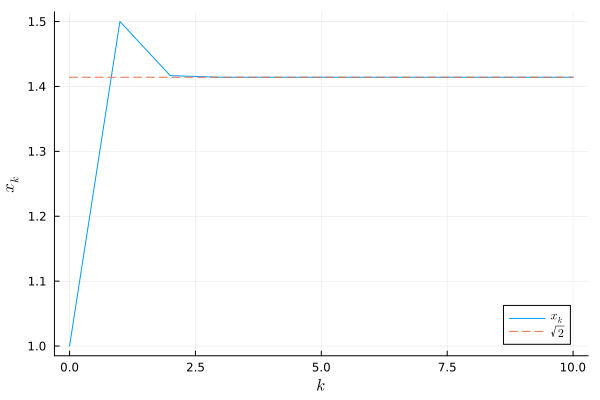
\includegraphics[scale=0.6]{question#2.png}
    \caption{$x_k$ vs. $\sqrt{2}$}
    \label{fig:my_label}
\end{figure}

\section*{Problem \#3}
Suppose we want to approximate the root of a function whose root is $2^{1/n}$, note that a simplified function that achieves such is,

\begin{equation*}
    g(x) = x^n - 2
\end{equation*}

and hence we compute,

\begin{equation*}
    g'(x) = nx^{n-1}
\end{equation*}

thus each $x^{(k+1)}$ for $k\in \NN$ is computed as,

\begin{equation*}
    x^{(k+1)} = x^{(k)} - \frac{(x^{(k)})^n-2}{n(x^{(k)})^{n-1}} = \frac{(n-1)x^{(k)}}{n} + \frac{2}{n(x^{(k)})^{n-1}}
\end{equation*}

\section*{Problem \#4}
Suppose we are given the following function of,

\begin{equation*}
    g(x) = x^5-2
\end{equation*}

such that,

\begin{equation*}
    g'(x) = 5x^4
\end{equation*}

then finding the root for $g(x)$, $2^{1/5}$ is denoted by,

\begin{equation*}
    x^{(k+1)} = x^{(k)} - \frac{g(x^{(k)})}{g'(x^{(k)})} = \frac{4x^{(k)}}{5} + \frac{2}{5(x^{(k)})^{4}}
\end{equation*}

with $x^{(0)} = 1$, then

\begin{table}[H]
    \centering
    \begin{tabular}{c|c}
        $k$ &  $x^{(k)}$ \\
        \hline{} 0 &  1\\
        1 & 1.2\\
        2 & 1.1529012345679013\\
        3 & 1.1487288865273251\\
        4 & 1.1486983566199584 \\
        5 & 1.1486983549970351\\
        6 & 1.1486983549970351\\
        7 & 1.1486983549970351\\
        8 & 1.1486983549970351\\
        9 & 1.1486983549970351\\
        10 &1.1486983549970351
        
    \end{tabular}
    \caption{Finding $2^{1/5}$ using Newton's Method}
    \label{tab:my_label}
\end{table}

\section*{Problem \#5}

\begin{figure}[H]
    \centering
    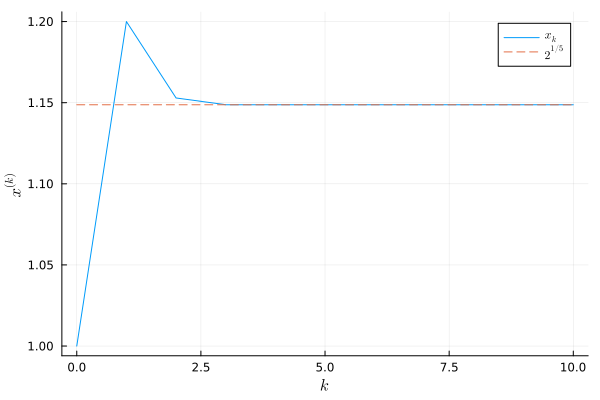
\includegraphics[scale=0.6]{question#5.png}
    \caption{$x^{(k)}$ vs. $2^{1/5}$}
    \label{fig:my_label}
\end{figure}

\section*{Problem \#6}
Suppose we are given the following function of,

\begin{equation*}
    g(x) = x^n-a
\end{equation*}

such that,

\begin{equation*}
    g'(x) = nx^{n-1}
\end{equation*}

then finding the root for $g(x)$, $a^{1/n}$ is denoted by,

\begin{equation*}
    x^{(k+1)} = x^{(k)} - \frac{g(x^{(k)})}{g'(x^{(k)})} = \frac{(n-1)x^{(k)}}{n} + \frac{a}{n(x^{(k)})^{n-1}}
\end{equation*}

\section*{Problem \#7}
Here we let $a = 8$ and $n = 3$, such that we want to approximate the root $8^{1/3}$, using the Newton Scheme above with $x_0 = 1$ we get,

\begin{table}[H]
    \centering
    \begin{tabular}{c|c}
        $k$ &  $x^{(k)}$ \\
        \hline{} 0 &  1\\
        1 & 3.3333333333333335\\
        2 & 2.4622222222222221\\
        3 & 2.0813412476715789\\
        4 & 2.0031374991412871 \\
        5 & 2.0000049116755041\\
        6 & 2.0000000000120624\\
        7 & 2.0000000000000000\\
        8 & 2.0000000000000000\\
        9 & 2.0000000000000000\\
        10 &2.0000000000000000
        
    \end{tabular}
    \caption{Finding $8^{1/3}$ using Newton's Method}
    \label{tab:my_label}
\end{table}


\section*{Problem \#8}
We compute the error for each $x^{(k)}$ as,

\begin{table}[H]
    \centering
    \begin{tabular}{c|c}
        $k$ &  $e^{(k)}$ \\
        \hline{} 0 &  1\\
        1 & 1.3333333333333335\\
        2 & 0.4622222222222221\\
        3 & 0.08134124767157891\\
        4 & 0.0031374991412871367 \\
        5 & 4.911675504093438e-6\\
        6 &  1.20623511179474e-11
\\
        7 & 0\\
        8 & 0\\
        9 & 0\\
        10 &0
        
    \end{tabular}
    \caption{Error for Approximating $8^{1/3}$ using Newton's Method}
    \label{tab:my_label}
\end{table}

\section*{Problem \#9}

Here we approximate $\pi$ by using the function,

\begin{equation*}
    g(x) = \tan(x)
\end{equation*}

and,

\begin{equation*}
    g'(x) = \sec^2(x)
\end{equation*}
then finding the root for $g(x)$, $\pi$ is denoted by,

\begin{equation*}
    x^{(k+1)} = x^{(k)} - \frac{g(x^{(k)})}{g'(x^{(k)})} = x^{(k)} - \frac{\tan(x)}{ \sec^2(x)} = x^{(k)} - \sin(x^{(k)})\cos(x^{(k)})
\end{equation*}

using $x^{(0)} = 3$ to get,

\begin{table}[H]
    \centering
    \begin{tabular}{c|c}
        $k$ &  $e^{(k)}$ \\
        \hline{} 0 &  3.0000000000000000\\
        1 & 3.1397077490994629\\
        2 & 3.1415926491252555\\
        3 & 3.1415926535897931\\
        4 & 3.1415926535897931 \\
        5 & 3.1415926535897931\\
        6 &  3.1415926535897931
\\
        7 & 3.1415926535897931\\
        8 & 3.1415926535897931\\
        9 &3.1415926535897931\\
        10 &3.1415926535897931
        
    \end{tabular}
    \caption{Approximating $\pi$ using Newton's Method}
    \label{tab:my_label}
\end{table}

\section*{Problem \#10}
We can do something similar to above for approximating $\pi$, by instead using

\begin{equation*}
    g(x) = \sin(x)
\end{equation*}

and,

\begin{equation*}
    g'(x) = \cos(x)
\end{equation*}
then finding the root for $g(x)$, $\pi$ is denoted by,

\begin{equation*}
    x^{(k+1)} = x^{(k)} - \frac{g(x^{(k)})}{g'(x^{(k)})} = x^{(k)} - \frac{\sin(x)}{ \cos(x)} = x^{(k)} - \tan(x^{(k)})
\end{equation*}

using $x^{(0)} = 3$ to get,

\begin{table}[H]
    \centering
    \begin{tabular}{c|c}
        $k$ &  $e^{(k)}$ \\
        \hline{} 0 &  3.0000000000000000\\
        1 & 3.1425465430742778\\
        2 & 3.1415926533004770\\
        3 & 3.1415926535897931\\
        4 & 3.1415926535897931 \\
        5 & 3.1415926535897931\\
        6 &  3.1415926535897931
\\
        7 & 3.1415926535897931\\
        8 & 3.1415926535897931\\
        9 &3.1415926535897931\\
        10 &3.1415926535897931
        
    \end{tabular}
    \caption{Approximating $\pi$ using Newton's Method}
    \label{tab:my_label}
\end{table}

\end{document}